\section{Convolutional Neural Networks for Risso’s Dolphins Identification}

\begin{center}
    \author{
    Rosalia Maglietta,
    Vito Renò,
    Rocco Cacioppoli,
    Emanuele Seller,
    Stefano Bellomo,
    Francesca Cornelia Santacesaria,
    Roberto Colella,
    Giulia Cipriano,
    Ettore Stella,
    Karin Hartman,
    Carmelo Fanizza,
    Giovanni Dimauro,
    \emph{(Member, IEEE)},
    Roberto Carlucci
    }
\end{center}

\begin{center}
    \emph{DIGITAL OBJECT IDENTIFIER}
\end{center}

\subsection{INTRODUCTION}
Photo identification is a technique that can be used on marine species in 
order to safeguard the environment and the various existing species. The 
marine species on which this study is based are cetaceans, in particular the 
Risso's dolphin species Grampus Griseus (Fig. \ref{fig:Risso}). This species is the least 
known and is present in greater numbers in Mediterranean waters. In order to 
recognize a dolphin, the scars present on their body and on the dorsal fin are 
used, representing the "fingerprints" useful for identifying them. To achieve 
this, the RUSPool algorithm is used which aims to perform an intelligent 
merge, through a custom filter, of the m RUSBoost classifiers. Subsequently, 
a new methodology called Neural Network Pool (NNPool) will be used, also 
useful for recognizing only the Risso species of dolphins. This algorithm is 
composed of a pool of CNNs useful for achieving the final goal. The chosen 
output will be dictated by the major voting of all these networks. Finally, 
the results obtained will be compared with those obtained by the RusPool 
algorithm, used for the same purpose.
\begin{figure}[h!]
    \centering
    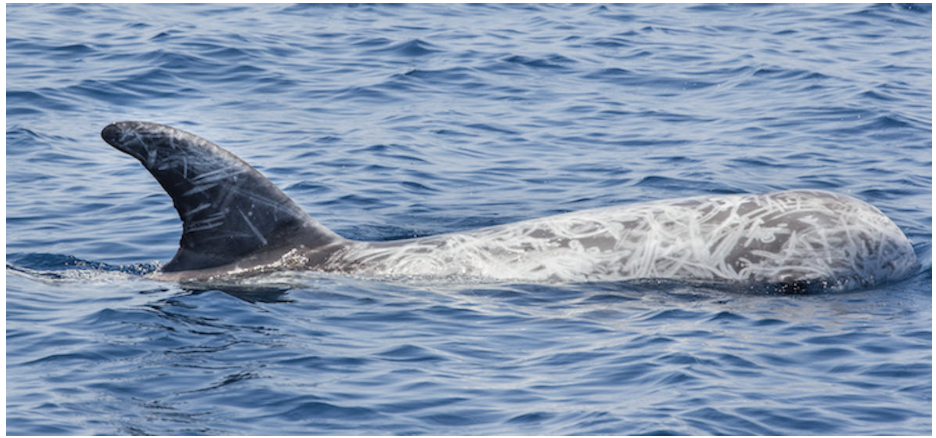
\includegraphics[width = 0.8\linewidth]{images/paper10/Risso.png}
    \centering
    \caption{Risso’s dolphins Grampus Griseus}
    \label{fig:Risso}
\end{figure}

\subsection{MATERIAL AND METHODS}
\subsubsection{Survey Area and Data Collection}
A dataset was created containing all the sightings of dolphins that took place 
in the years between 2013 and 2018, in the Gulf of Taranto. The collection 
contains a total of 93 different labeled Risso dolphins, but sadly only 23 of 
these were selected as each has at least 15 images on each side of the fin. 
Through the use of an $f_R$ mask filter, 70\% of each image consists of the 
dolphin fin alone, excluding external elements such as the sea. This filter 
led to consider a new dataset $D_R$ containing 433 images belonging to the 23 
dolphins. The $D_{NN}$ dataset used to train CNNs contains images that have 
not been pre-processed by the $f_R$ filter. This latest dataset is made up of 
582 images belonging to 28 different dolphins. A validation dataset was also 
created containing 300 images of known and unknown Risso's dolphins.

\subsubsection{RUSBoost Methodology}
The RUSBoost algorithm has the task of identifying each dolphin and predicting 
its label. The application of this algorithm can be schematized in 
figure \ref{fig:RUSBoost}. The architecture consists of 3 main phases:
\begin{enumerate}
    \item \emph{Pre-processing}: creation of the black and white image containing the 
    extracted fin.
    \item \emph{Features Extraction}: build the 3-dimensional super-SIFT descriptor. 
    \item \emph{Classification}: application of the RUSBoost algorithm.
\end{enumerate}
RUSBoost consists of two other types of algorithms: Random Under-Sampling 
(RUS) and Adaboost \cite{0907875811}. RUSBoost training takes place by carrying out 
cross-validation, one against all, on each of the 23 dolphins taken into consideration, 
therefore $M_i$ classifiers will be created, with $i = 1,2,...,23$.
\begin{figure}[h!]
    \centering
    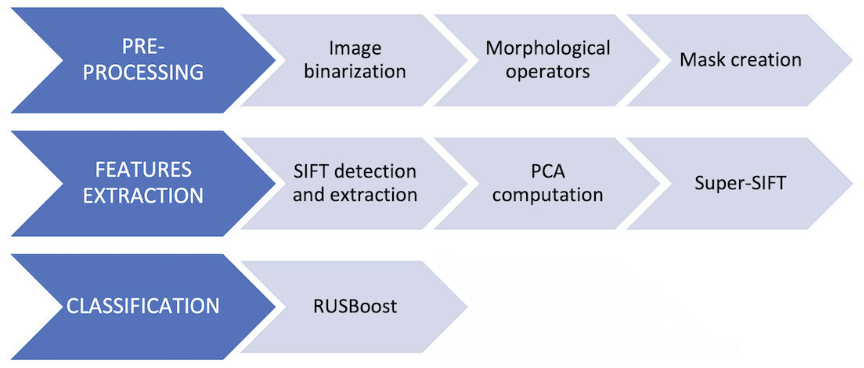
\includegraphics[width = 0.8\linewidth]{images/paper10/RUSBoost.png}
    \centering
    \caption{Experimental methodology based on RUSBoost.}
    \label{fig:RUSBoost}
\end{figure}

\subsubsection{RUSPool}
The RUSPool algorithm aims to identify known dolphins among all and unknown 
ones. This task is done by using the previous 23 already trained 
RUSBoosts classifiers (Fig. \ref{fig:RUSPool Arch}). Therefore, each image given as input to RUSPool 
will have n super-SIFT descriptors associated with it and this new sample is 
supplied as input to the RUSBoosts classifiers. The result returned by each 
classifier will represent the prediction that a dolphin has been recognized or 
not. The result obtained from the difference in these probabilities, if greater 
than a threshold equal to $0.11$, will be taken into consideration, discarding 
all other cases of uncertainty. The final output will be a vector $R$ where its 
elements $r_i$ represent the percentage of positive predictions for each classifier 
$M_i$ (Fig. \ref{fig:ri}). A filter is applied on the vector R to obtain the 
prediction of the identity of a dolphin given in input.
\begin{figure}[h!]
    \centering
    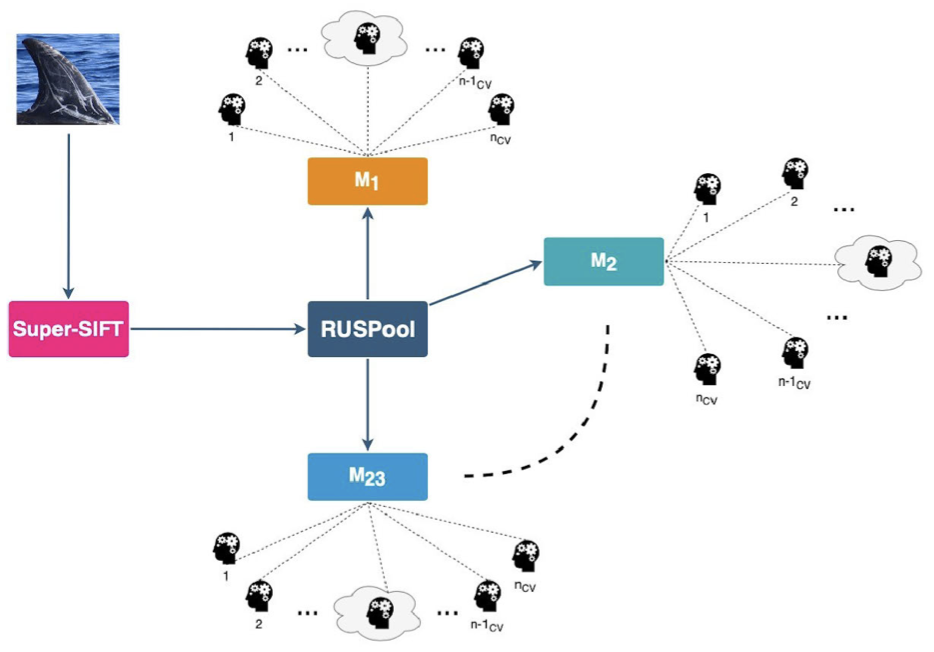
\includegraphics[width = 0.5\linewidth]{images/paper10/RUSPool Architecture.png}
    \centering
    \caption{RUSPool Architecture.}
    \label{fig:RUSPool Arch}
\end{figure}
\begin{figure}[h!]
    \centering
    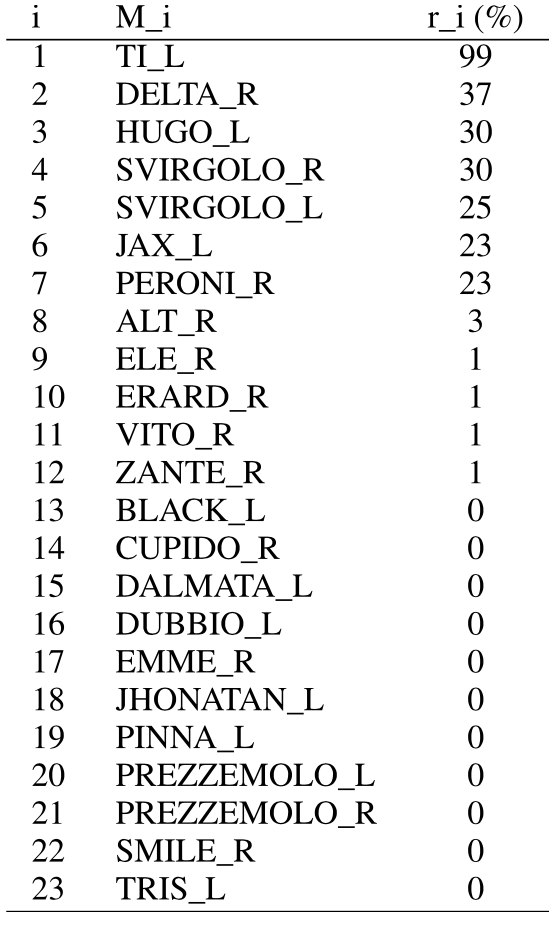
\includegraphics[width = 0.4\linewidth]{images/paper10/ri.png}
    \centering
    \caption{Example of RUSPool output. $r_i$ is the bumber of positive predicitons of the $M_i$ classifiers.}
    \label{fig:ri}
\end{figure}

\subsubsection{Convolutional Neural Network}
A convolutional neural network (CNN) is used. Its architecture is composed 
of a triple sequence of Conv-ReLu-MaxPool layers (Fig. \ref{fig:CNNDol}). The number of 
parameters and images useful for training the network is less than the most 
widespread neural networks in the state of the art, thus reducing the problem 
of overfitting. This architecture forms the previous NNPool network. The 
dataset used is the one previously mentioned DNN.
\begin{figure}[h!]
    \centering
    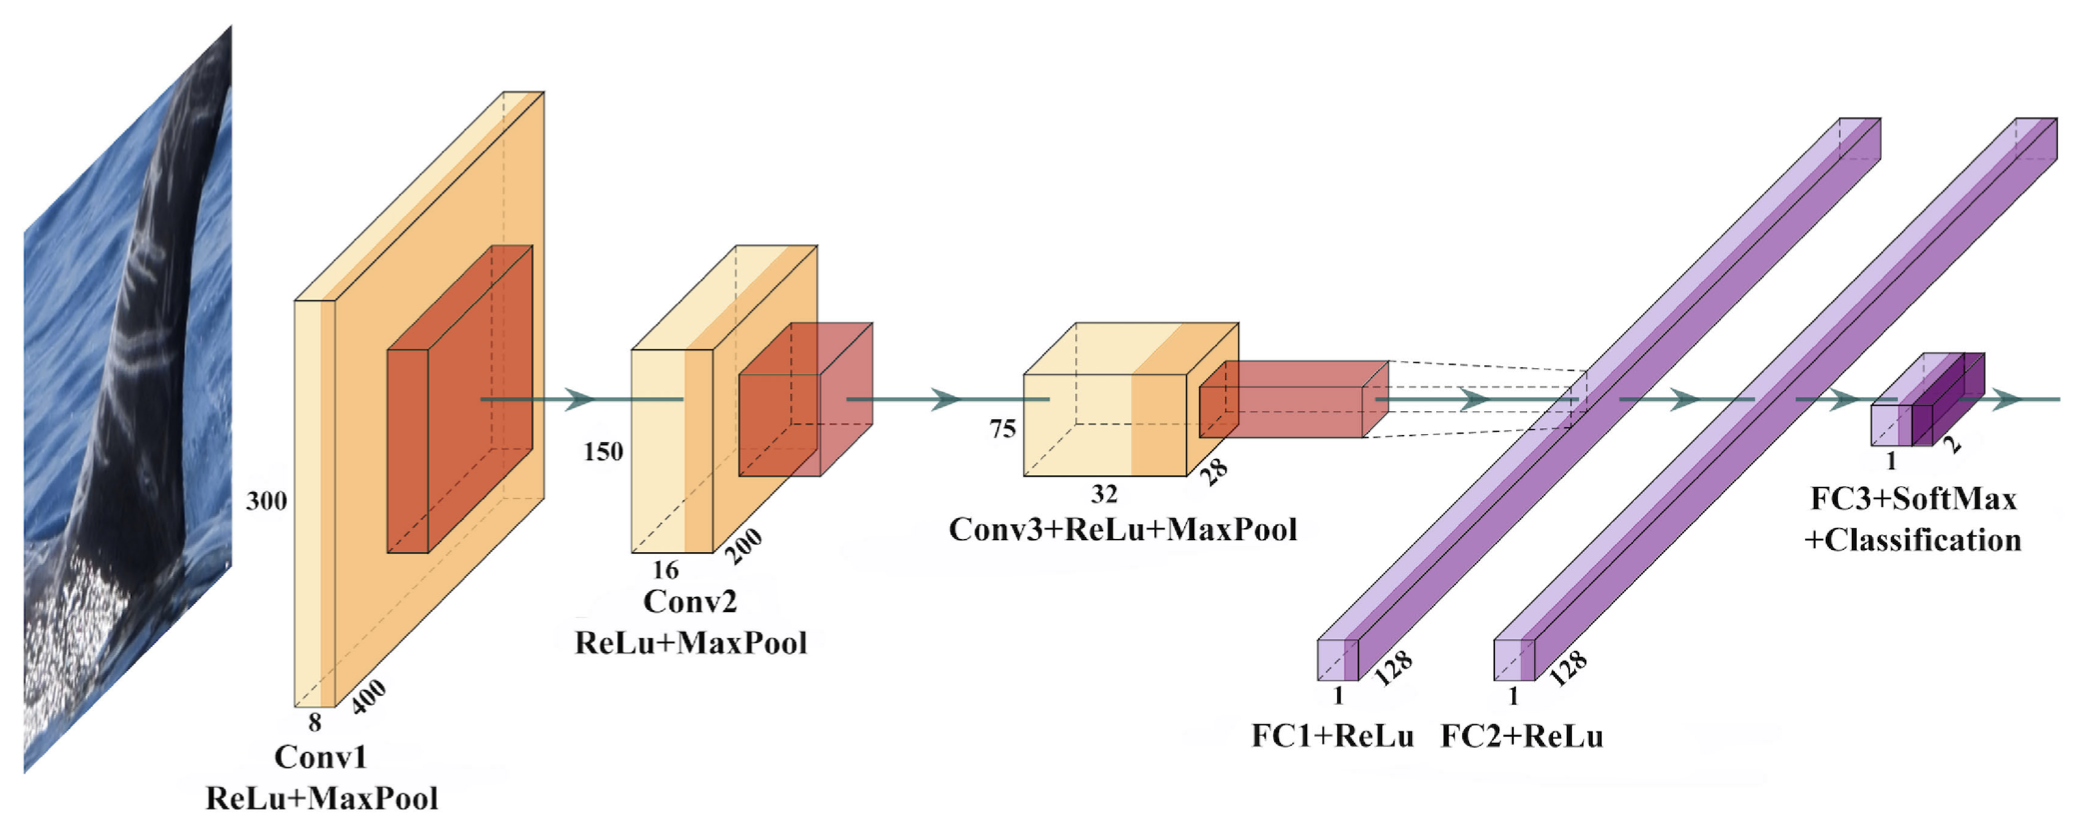
\includegraphics[width = 0.7\linewidth]{images/paper10/NNPool Architecture.png}
    \centering
    \caption{CNN Architecture build for each dolphin.}
    \label{fig:CNNDol}
\end{figure}

\subsubsection{NNPool}
The proposed strategy is called NNPool. This strategy is based on the composition 
of several CNN networks equal to the number of dolphins present in 
the $D_{NN}$ dataset. The output generated by NNPool is a probability vector \emph{P} 
(Fig. \ref{fig:NNPool output}) where, if there is only one probability $p_i\in P > 51\%$ , then the new 
photo given in input will be labeled as known, otherwise it will be labeled as 
unknown.
\begin{figure}[h!]
    \centering
    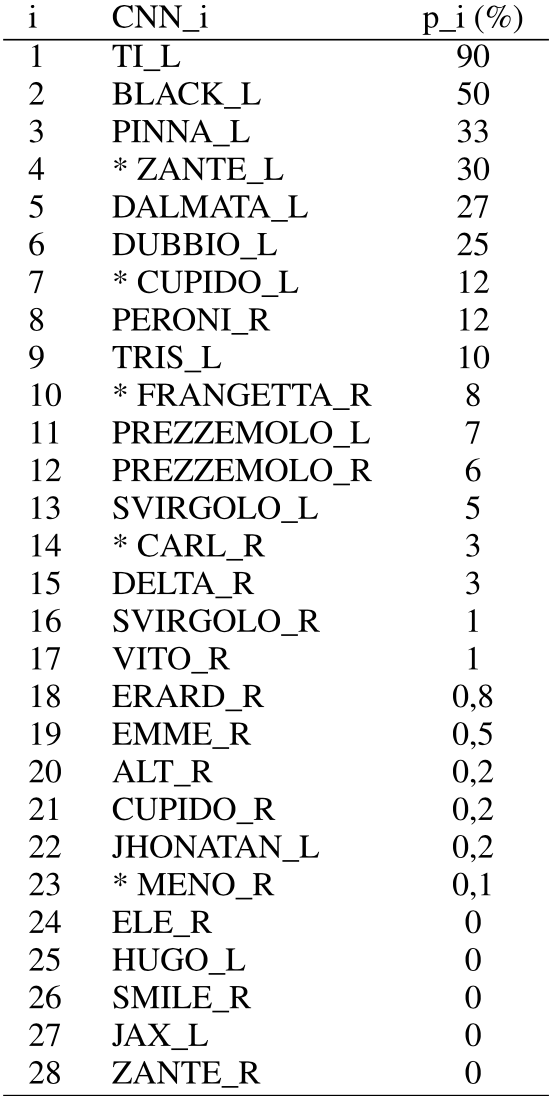
\includegraphics[width = 0.4\linewidth]{images/paper10/NNPool output.png}
    \centering
    \caption{Example of NNPool output. $p_i$ is the probabilities of the fin given in input to belong to the dolphin reported to the $CNN_i$.}
    \label{fig:NNPool output}
\end{figure}

\subsubsection{Evaluation Metrics}
The metrics used to evaluate the performance of the proposed model are as follows:
\begin{enumerate}
    \item \emph{Accuracy}: percentage of correct predictions.
    \item \emph{Sensitivity}: percentage of positive labels considered as positive.
    \item \emph{Specificity}: percentage of negative labels considered as negative.
\end{enumerate}
Images labeled as negative will correspond to unknown classes.

\subsection{EXPERIMENTS AND RESULTS}
To compare the results obtained by NNPool you must first create the RUSBoost 
model. This model uses the $D_R$ dataset on which the Cross-Validation 
technique is used to train the model. The quality of each image can affect 
the model. To solve this problem, a method called Perception based Image 
Quality Evaluator (PIQE scores) is used which determines the type of quality 
(Excellent, Good, Fair, Poor, Bad) based on the score obtained on each 
image (Low is better). The results obtained by RUSBoost are those shown 
in figure \ref{fig: RUSBoostPerf}. Unfortunately, the performance of RUSBoost depends on 
the number of images available for training and the quality of each of them. The 
RUSPool model is then created to compare its performance. This time the 
$D_v$ dataset is used. The accuracy, sensitivity and specificity values achieved 
are visible in table \ref{RUSPoolPerf}. At this point, the performance of CNN networks on 
the $D_{NN}$ dataset is also evaluated. To evaluate the performance of a CNN 
network, and therefore of NNpool, the Cross-Validation strategy is used with 
a number of $n_{cv}$ cycles equal to 10 on a dataset divided into 2/3 of training 
set and 1/3 of test set. The results are averaged across all the $n_{cv}$. Figure \ref{fig: CNNNNPool perfromance} 
shows the results obtained by every CNN network of NNPool which demonstrate 
its superiority over RUSBoost. Since there are dolphins made up of 
a different number of images, when the quantity of images exceeds 3.5\% the 
sensitivity increases, otherwise it decreases. The strong point of the CNN 
network is that it achieves good performance both in case there are many 
low quality images and in case there are few high quality images. As for the 
performances achieved by NNPool, these exceed that of RUSPool. Also regarding 
the training and classification time (recognition of a single unknown 
image), NNPool is less time-consuming than RUSPool.
\begin{figure}[h!]
    \centering
    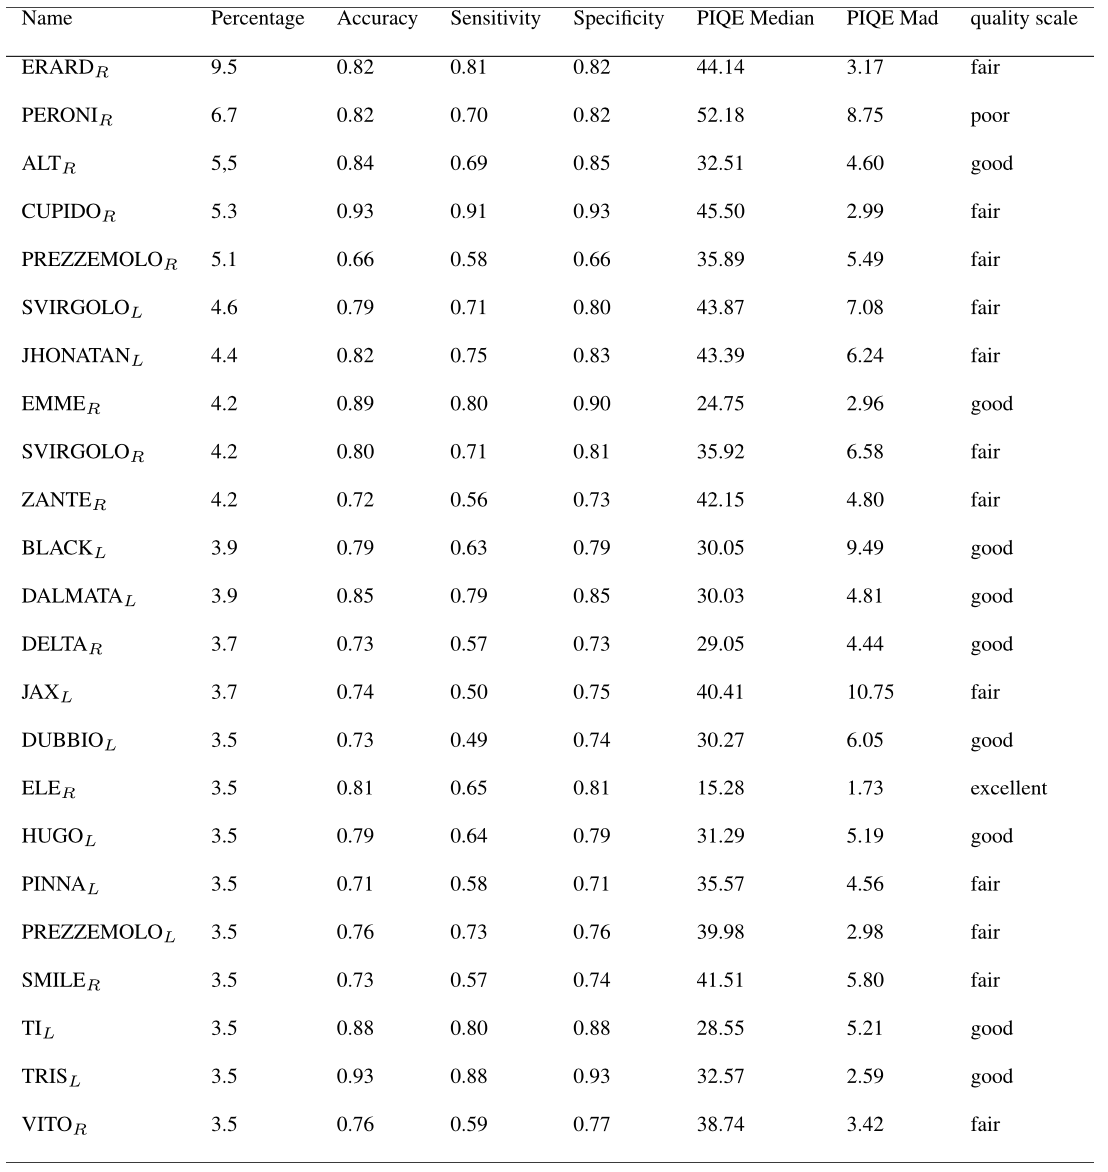
\includegraphics[width = 0.8\linewidth]{images/paper10/RUSBoost performance.png}
    \centering
    \caption{Performances of RUSBoost.}
    \label{fig: RUSBoostPerf}
\end{figure}
\begin{table}[htbp]
    \centering
    \begin{adjustbox}{width=0.7\textwidth}
    \begin{tabular}{|cccc|}
        \hline
        & Accuracy & Sensitivity & Specificity\\
        \hline
        RUSPool & 0.78 & 0.58 & 0.81\\
        NNPool & 0.87 & 0.70 & 0.90\\
        \hline
    \end{tabular}
    \end{adjustbox}
    \caption{RUSPool and NNPool performance on the validation data set $D_v$}
    \label{RUSPoolPerf}
\end{table}

\begin{figure}[h!]
    \centering
    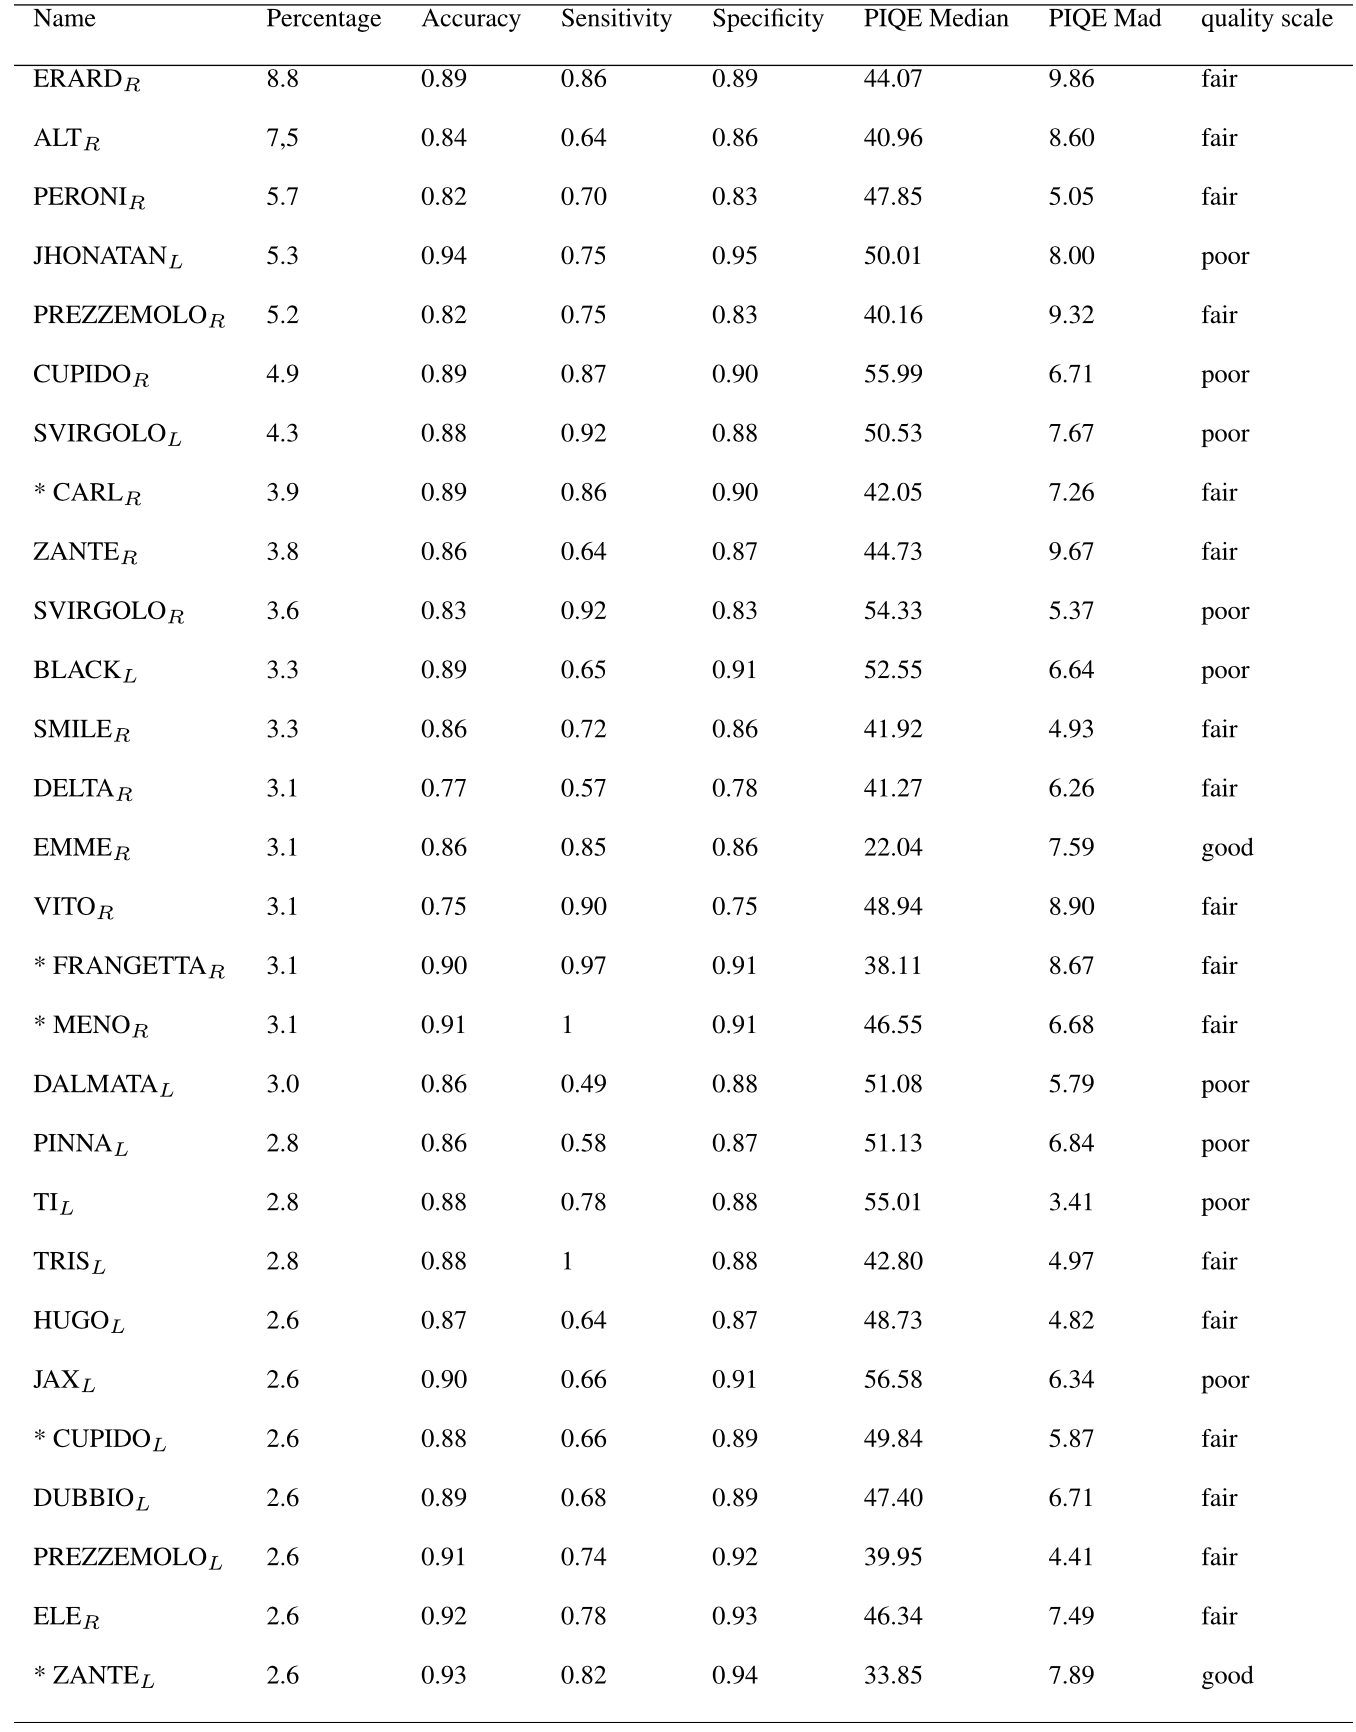
\includegraphics[width = 0.8\linewidth]{images/paper10/NNPool performance.png}
    \centering
    \caption{Performances of every CNN network in NNPool.}
    \label{fig: CNNNNPool perfromance}
\end{figure}

\subsection{CONCLUSION}
In conclusion, it can be said that, among all the methods compared, the 
proposed CNN network has better performances and more advantages. One 
of the first is the non-interaction of the user, while following there is the factor 
of the training and classification speed. Unfortunately, like many CNN-based 
methods, the problem of the number of images, and their quality, still remains 
open in fact by providing a low number of images, all with low quality, the 
proposed algorithm will tend to have low performance in terms classification 
of dolphins.

